\section{Results}

\subsection*{Surprising Language and User Behavior}

The distribution of cross-entropy for each period is fairly similar -- we notice each distribution is fat-tailed and the mean cross-entropy is stable. Period 10, the month of the election, has the highest average cross-entropy. There does not seem to be any variation with time. From Figure \ref{fig:ce_stats}, we also notice that there is no relationship between the cross-entropy and score of a post, and that the relationship between cross-entropy and the number of comments is weak. Thus, filtering on these two parameters would not be equivalent to selecting on the outcome. 

To understand the influence of top users, I plot the average cross-entropy of their posts against that of the community in  Figure \ref{fig:ce_comp}. Top users are defined as those who have made at least 5 posts per period, and whose posts have a mean score greater than 2500 -- regular users whose posts get consistently high scores, about the top 3\% of posters and 10\% of posts. We notice that the cross-entropy of these top users is highly correlated to that of the community at every period, indicating they do not have wildly different language usage from the community. Additionally, we observe that the average cross-entropy of these users is less than the average of the community, i.e. their language is less surprising. This could be an indicator that these users embody the norms of the community, and are thus able to command attention. 

% Cross-Entropy Distribution
\begin{figure}[h]%

    \centering

    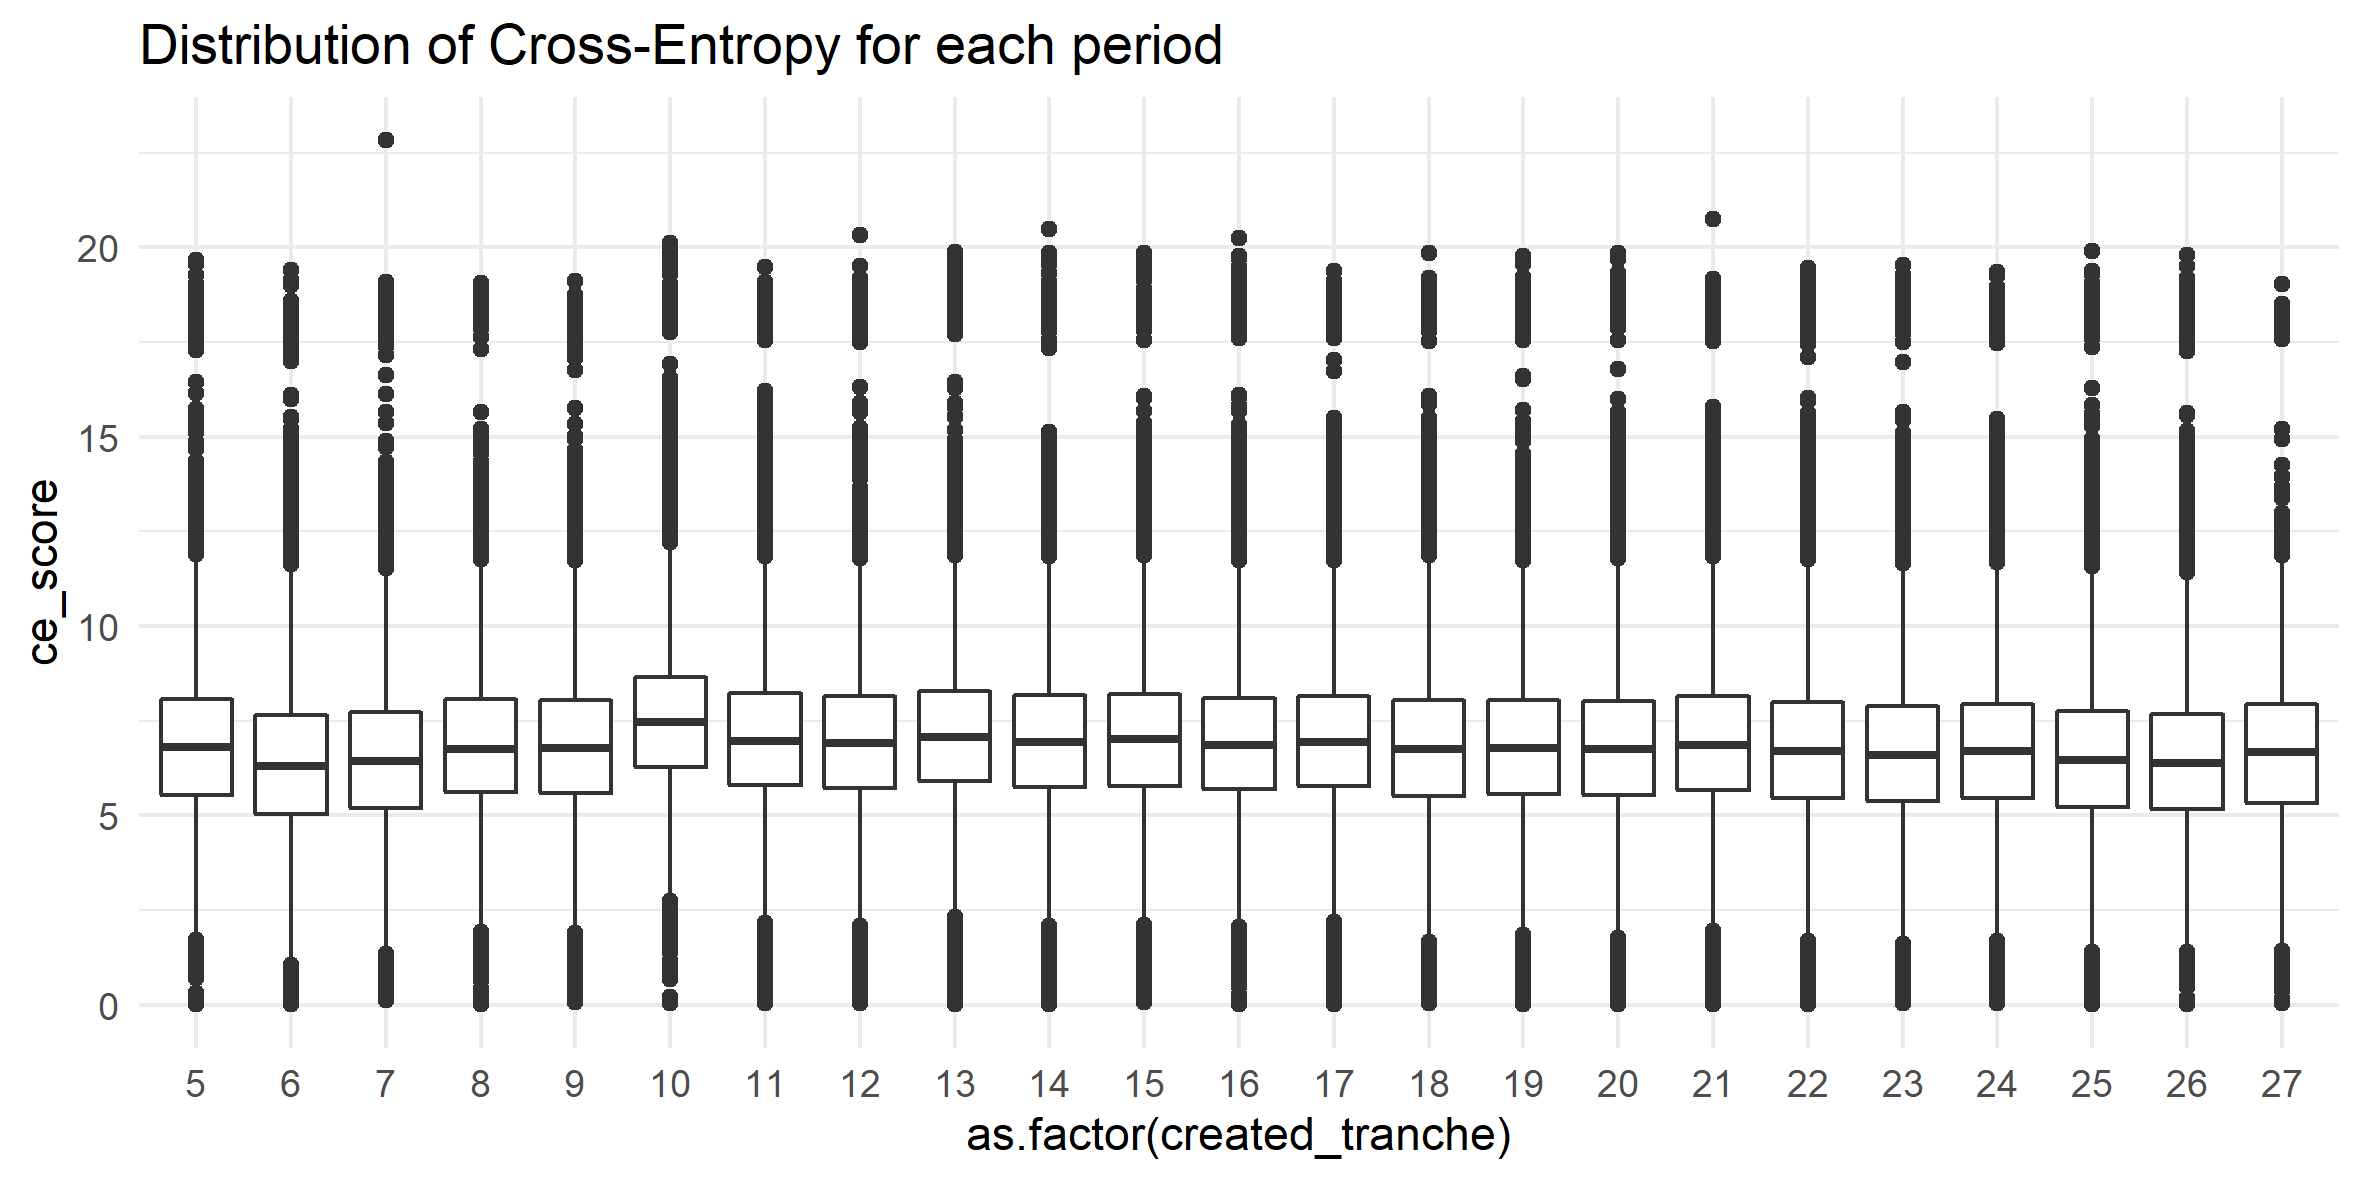
\includegraphics[width=0.8\linewidth]{figures/ce_boxplot.png}
    \caption{Distribution of Cross-Entropy for each 6-week period.}%

    \label{fig:ce_boxplot}%

\end{figure}

% Entropy vs score and comments
\begin{figure}[h]%

    \centering

    \subfloat[Entropy-vs-Score]{{ 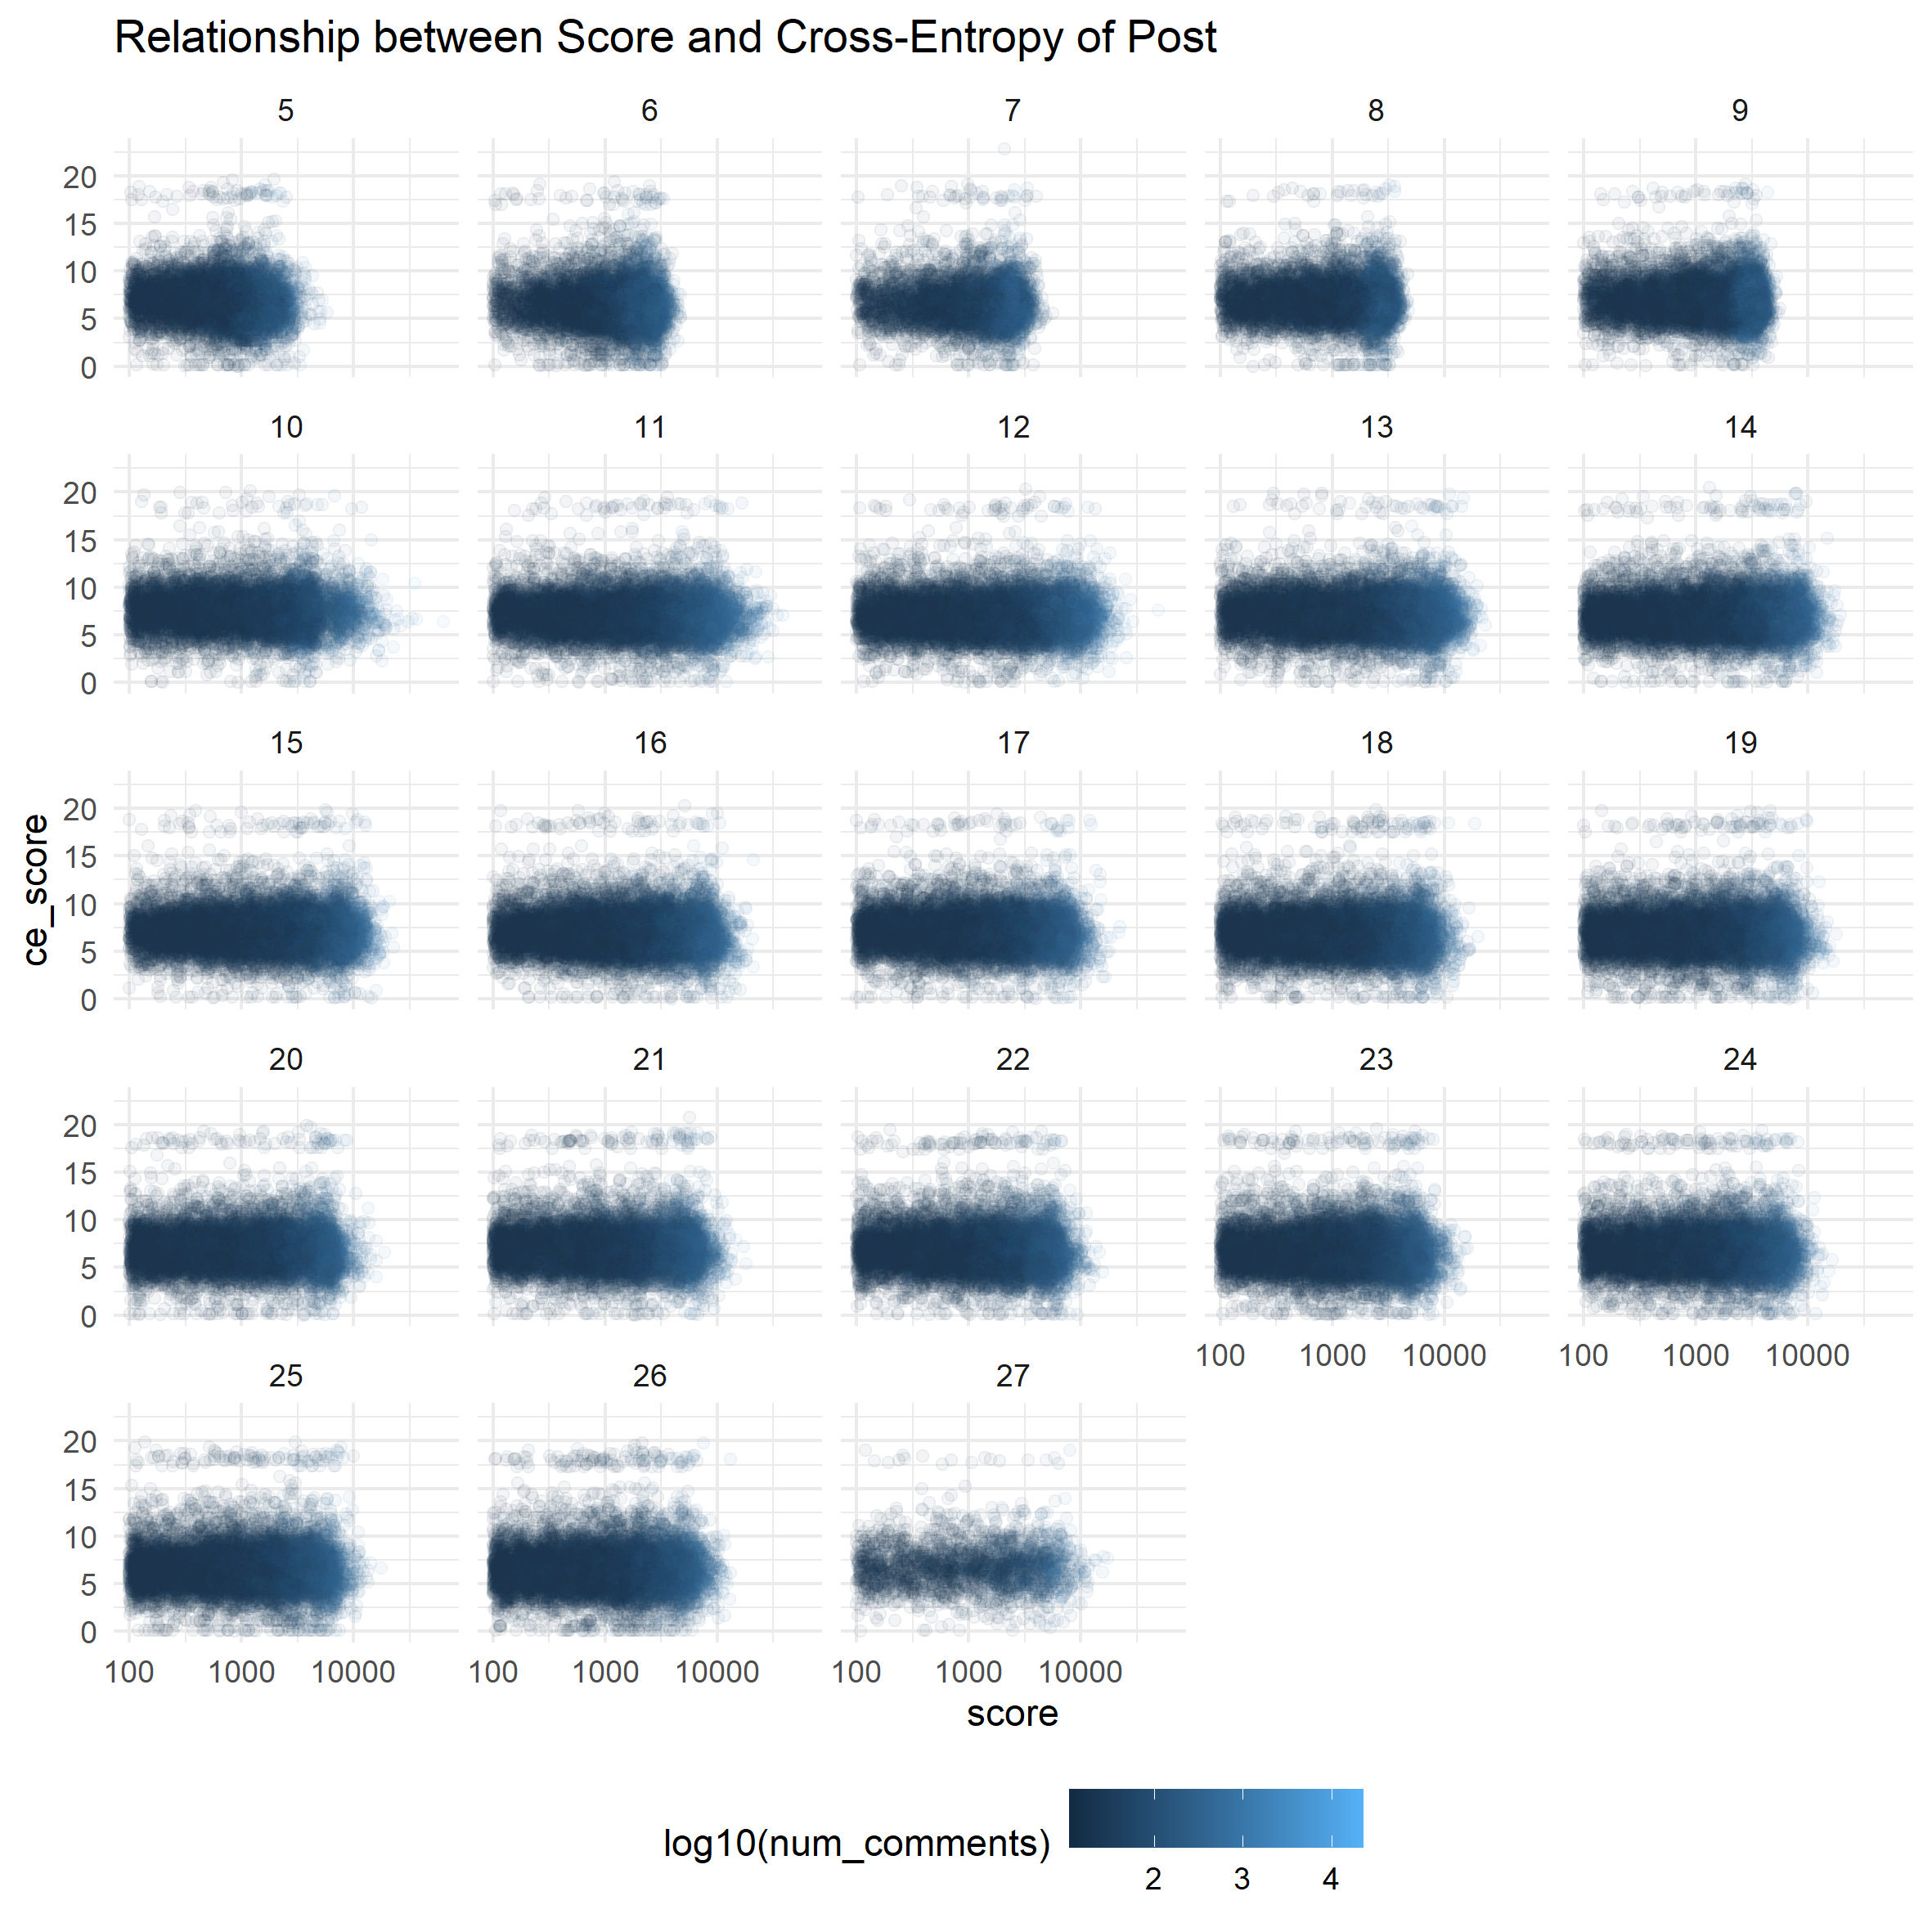
\includegraphics[width=0.45\linewidth]{figures/score_ce_plot.png}}} ~
    \subfloat[Entropy-vs-Comments]{{ 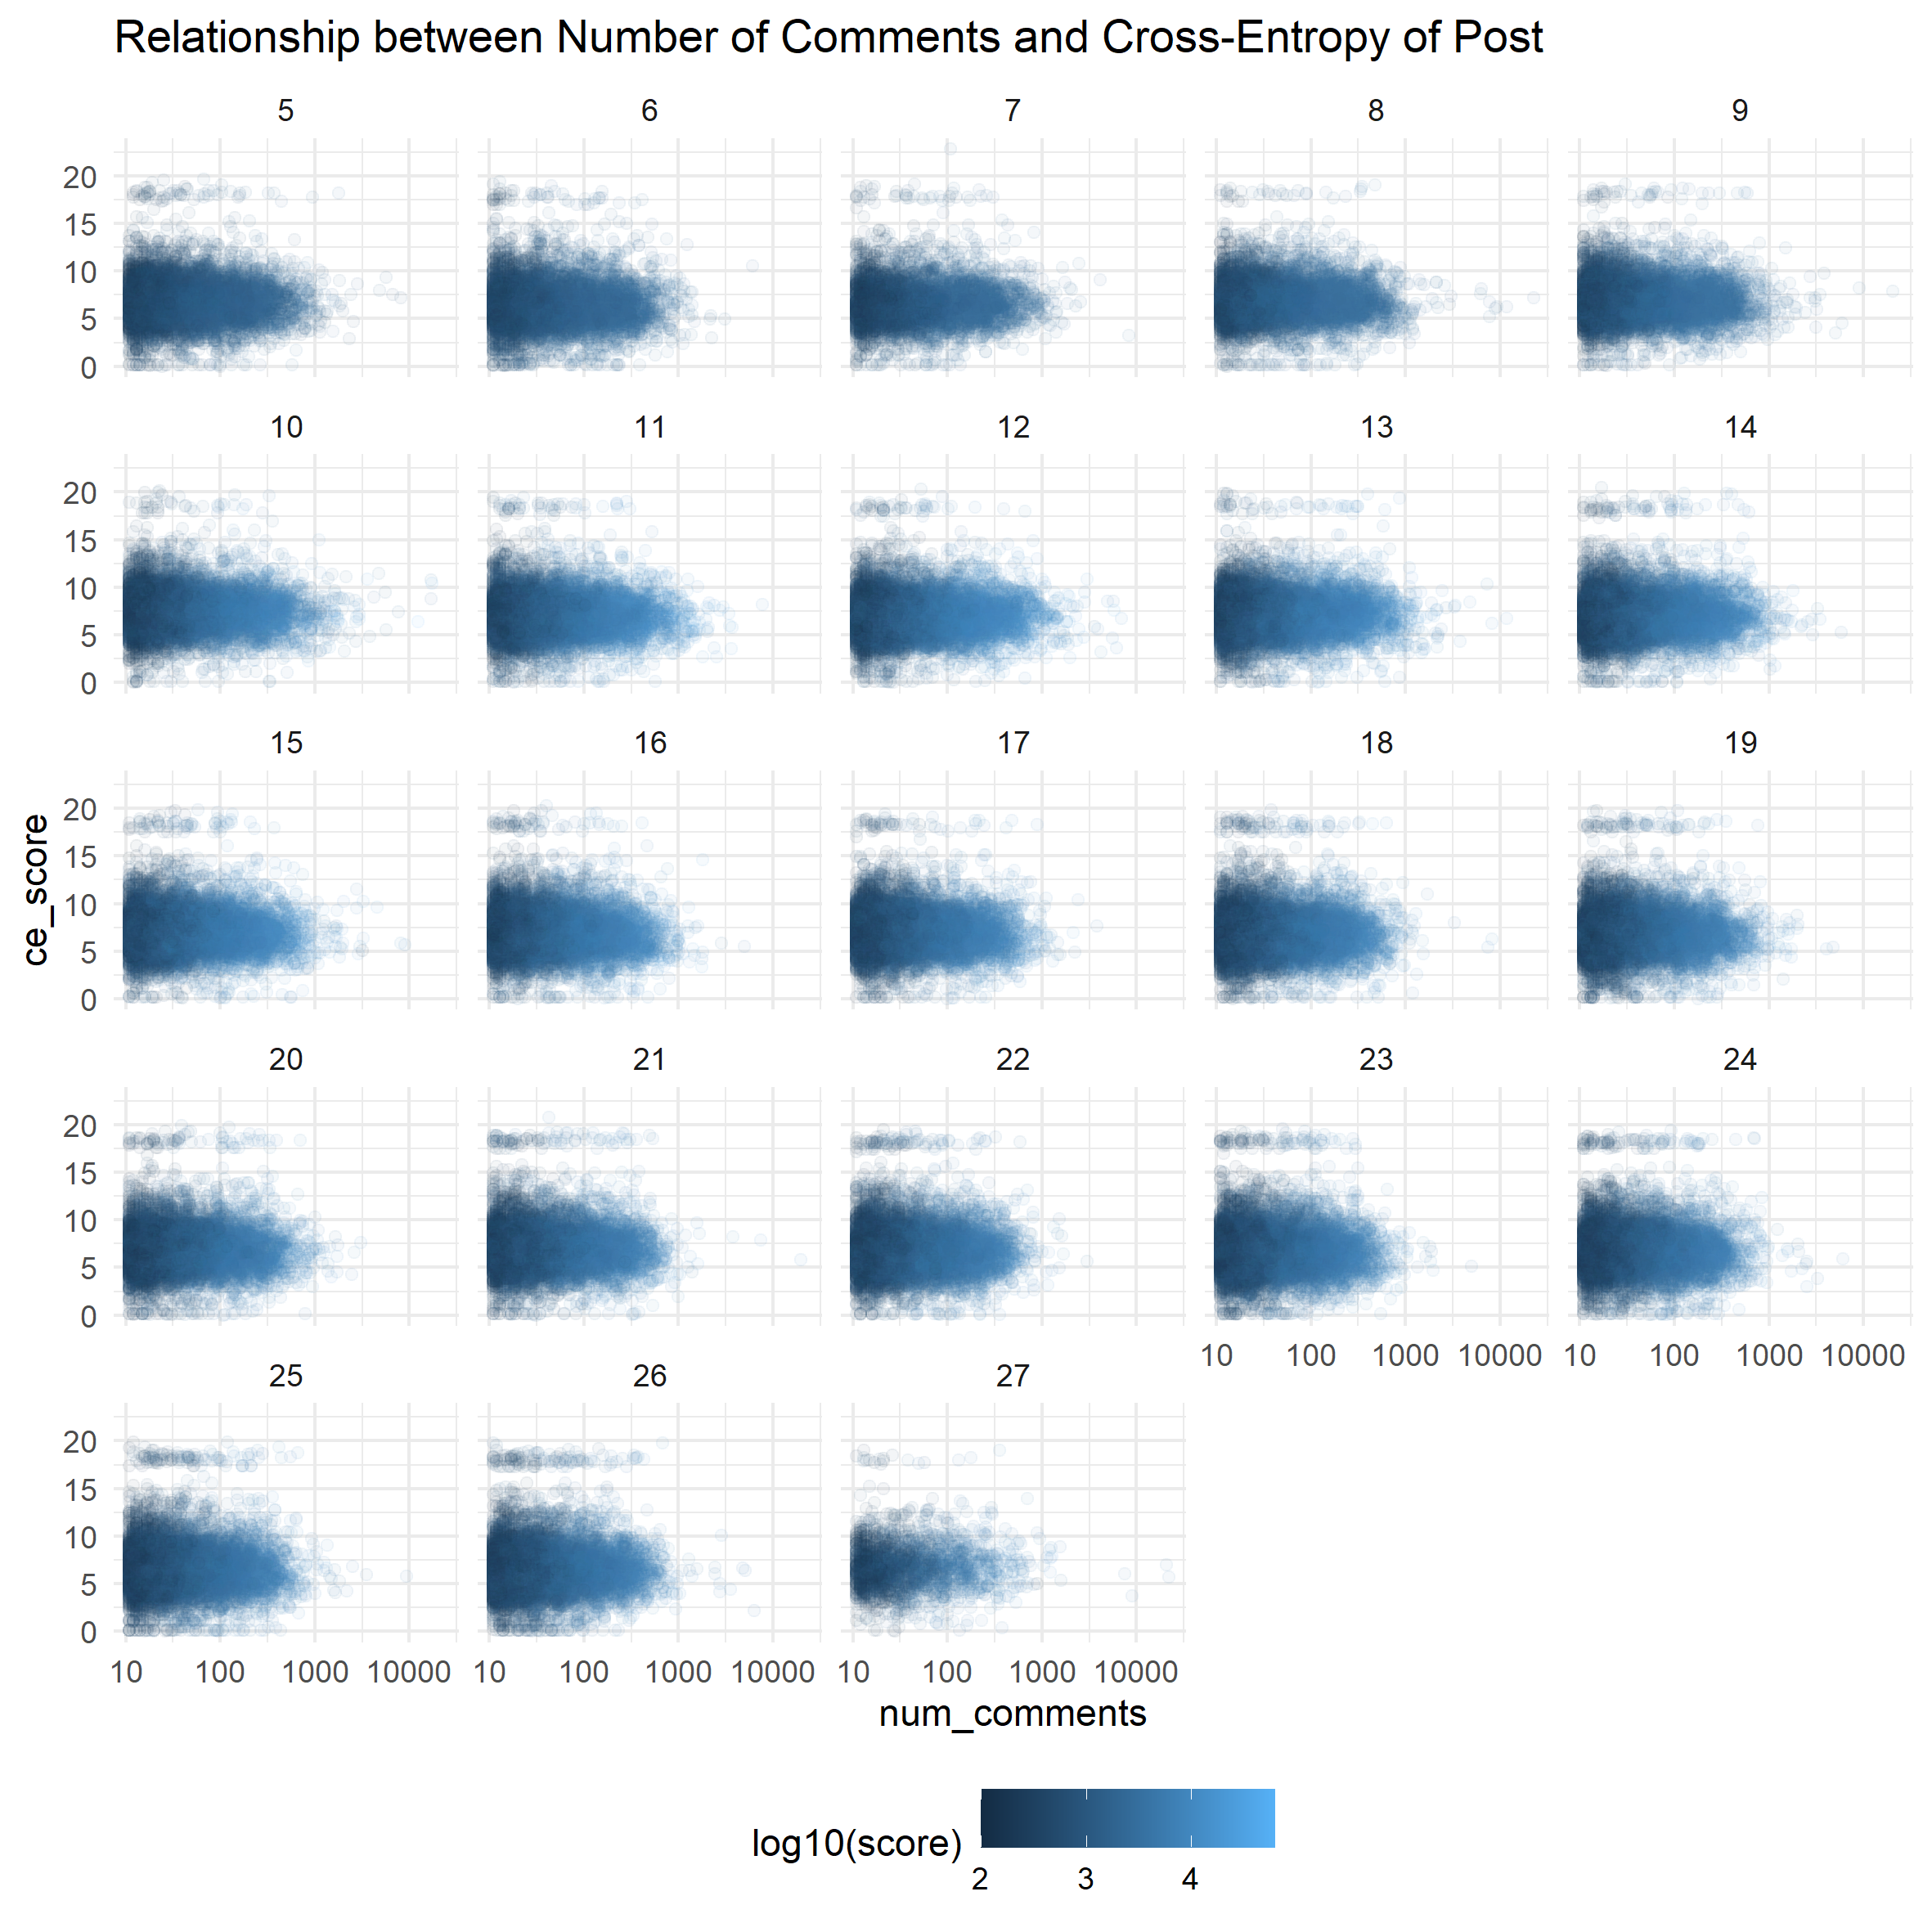
\includegraphics[width=0.45\linewidth]{figures/comm_ce_plot.png} }}
    
    \caption{Relationship between Cross-Entropy and Score, Number of Comments.}%

    \label{fig:ce_stats}%

\end{figure}


% Cross-Entropy of top-users
\begin{figure}[h]%

    \centering

    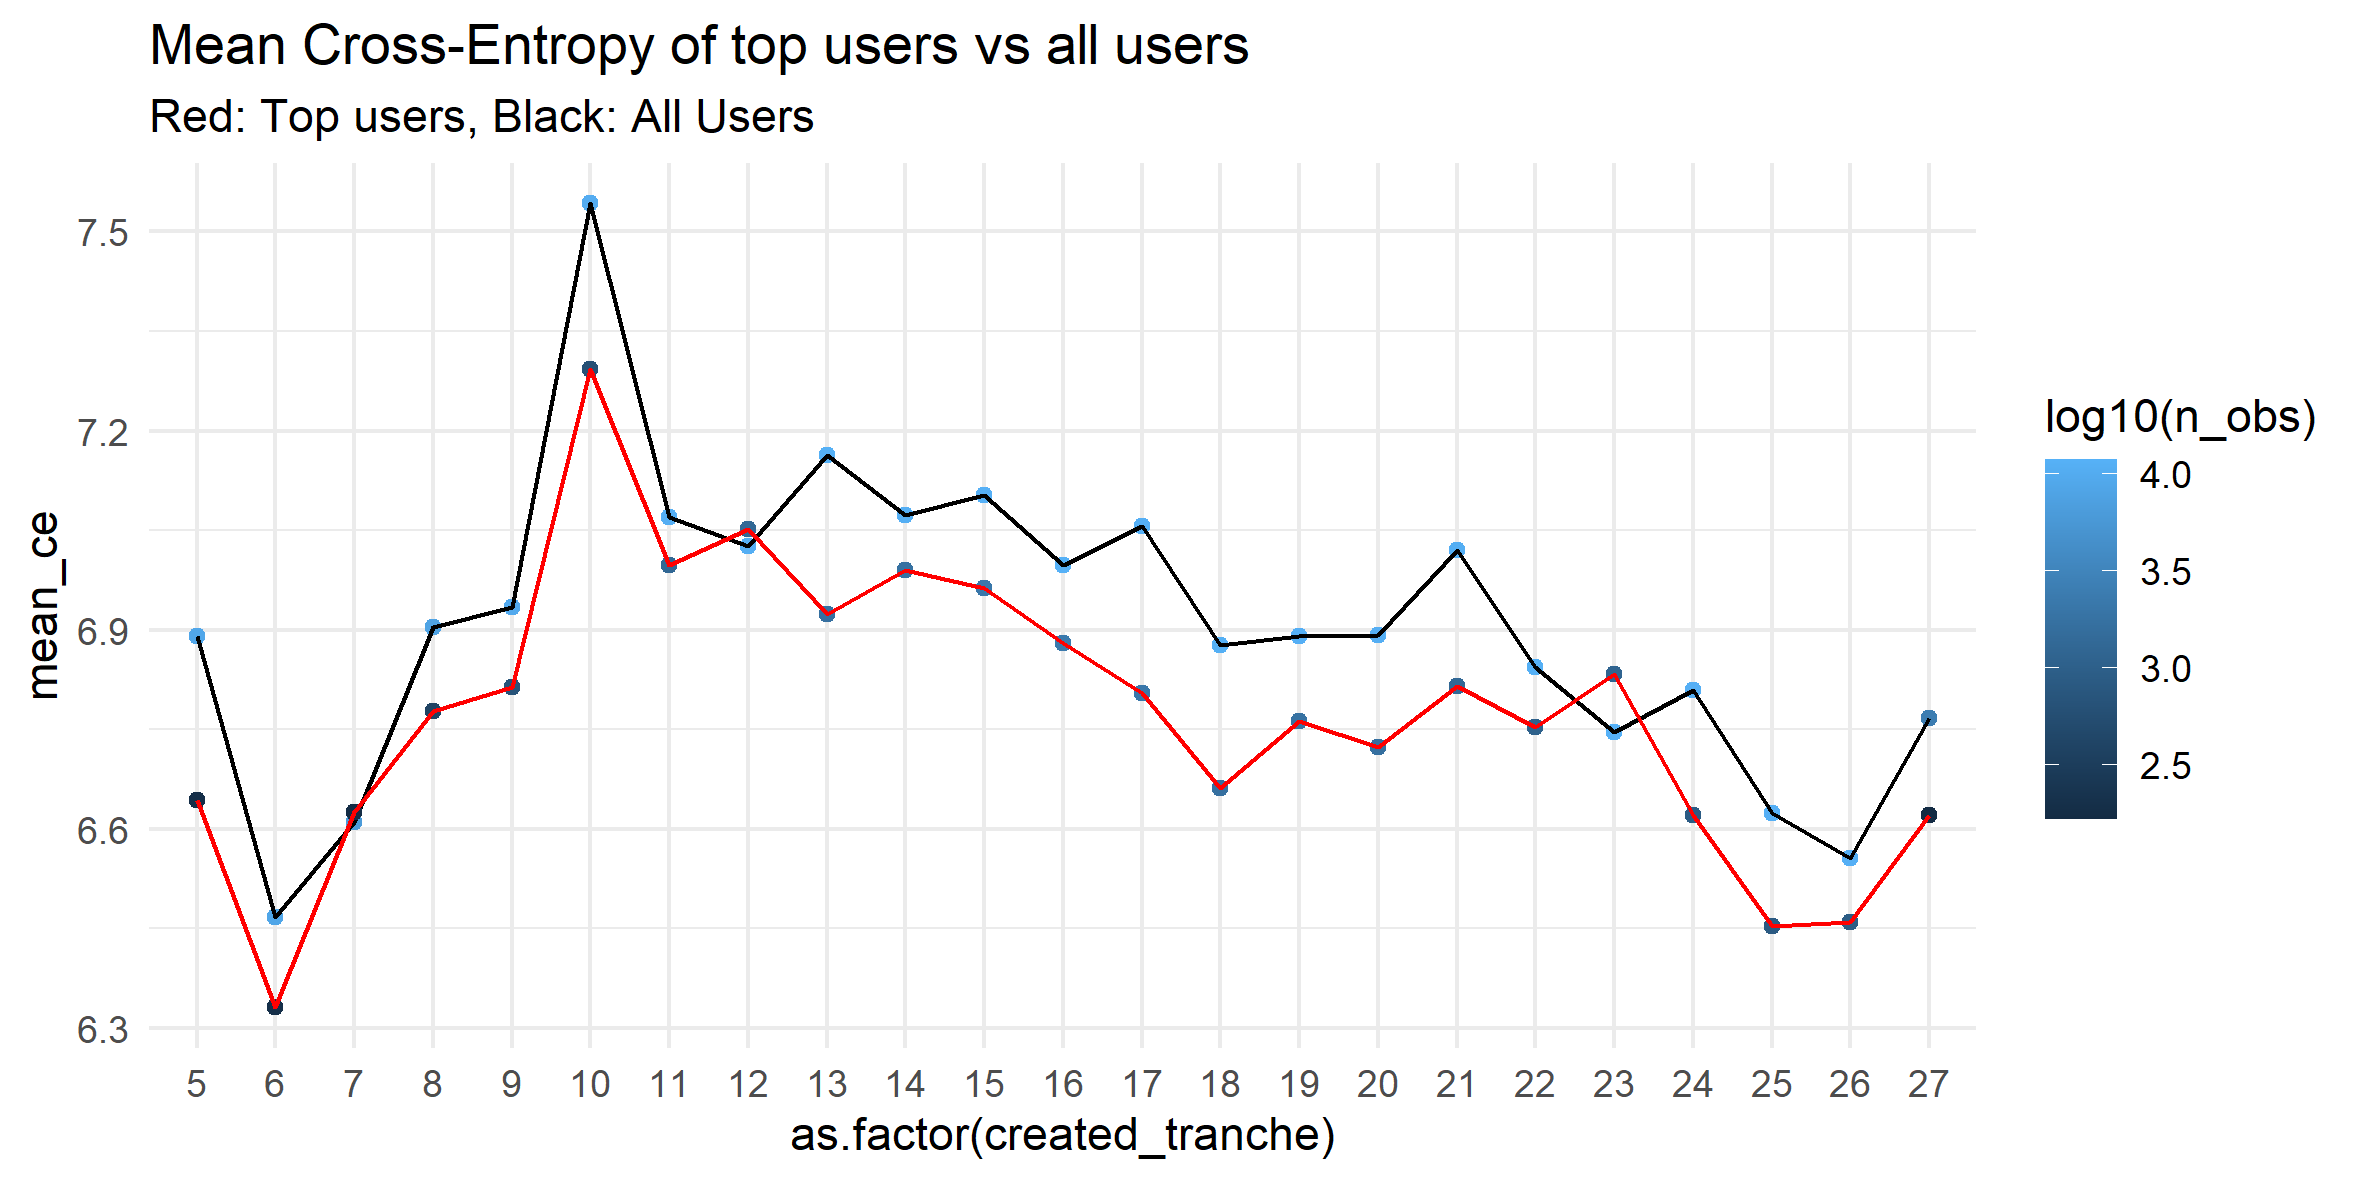
\includegraphics[width=\linewidth]{figures/comp_ce_plot.png}
    \caption{Mean Cross-Entropy of all posts vs top users for each 6-week period.}%

    \label{fig:ce_comp}%

\end{figure}



\clearpage
\subsection*{Using Divergence measures to identify a change in context}

\subsubsection*{Immigration policies}

% Divergence of Immigration
\begin{figure}[t]%

    \centering

    \subfloat[`immigrant']{{ 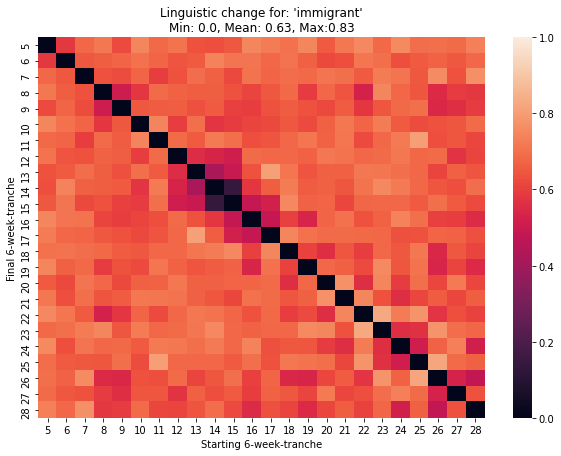
\includegraphics[width=0.32\linewidth]{figures/div_graphs/immigrn-immigrant.png} }} ~
    \subfloat[`border']{{ 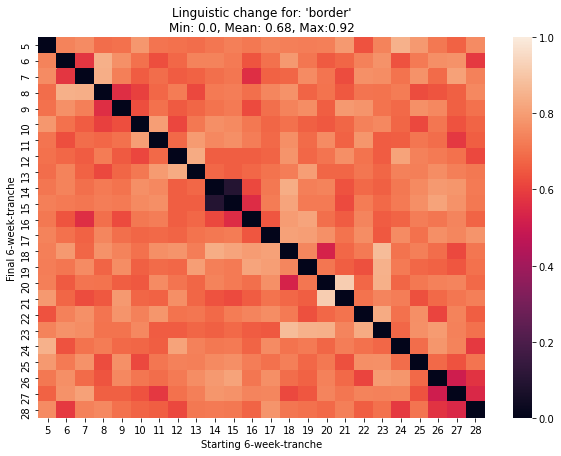
\includegraphics[width=0.32\linewidth]{figures/div_graphs/immigrn-border.png} }} ~
    \subfloat[`separation' (Family Separation policy)]{{ 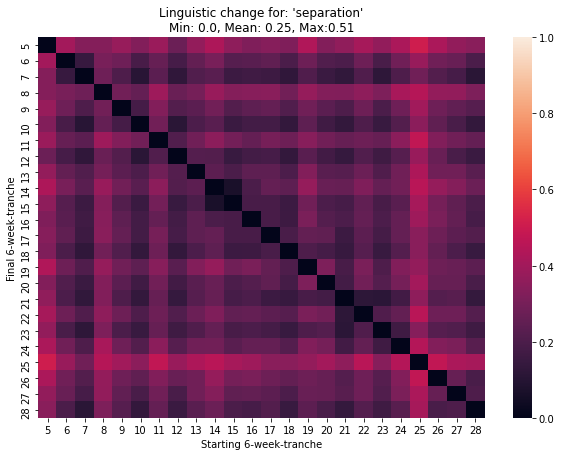
\includegraphics[width=0.32\linewidth]{figures/div_graphs/scandal-separation.png} }}
    
    \subfloat[`hispanic']{{ 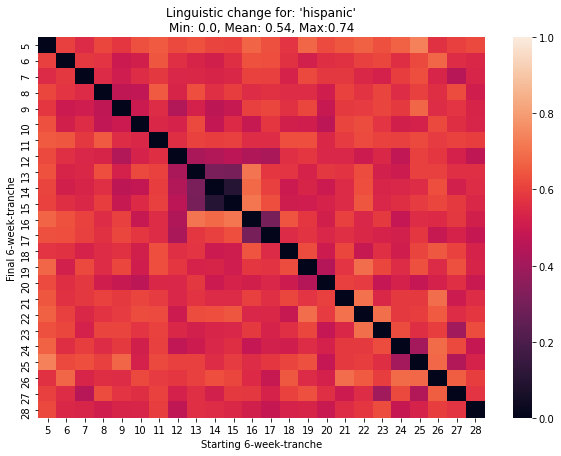
\includegraphics[width=0.32\linewidth]{figures/div_graphs/immigrn-hispanic.png} }} ~
    \subfloat[`mexican']{{ 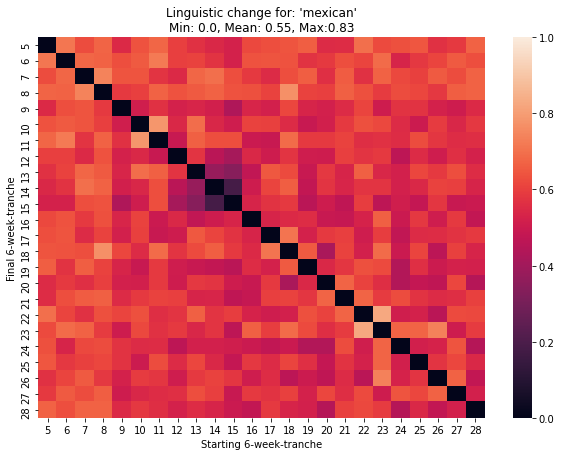
\includegraphics[width=0.32\linewidth]{figures/div_graphs/immigrn-mexican.png} }}~
    \subfloat[`muslim']{{ 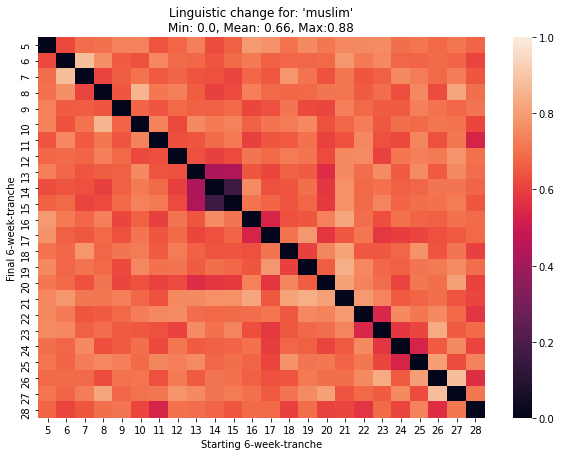
\includegraphics[width=0.32\linewidth]{figures/div_graphs/immigrn-muslim.png} }}
    
    \caption{Relative Divergence of words related to Trump's Immigration policies using aligned word embeddings.}%

    \label{fig:div_immigr}%

\end{figure}

Immigration was and continues to remain a cornerstone of President Trump's legislative agenda. The first notes of stabilization for \texttt{immigrant, border} begin in period 12 in the early months of the presidency, as we see in Figure \ref{fig:div_immigr}. The thrust on immigration continues until period 17, before it picks up again during periods 22. This later spike is associated with the legislative focus on the border family separation issue. The community's context around \texttt{separation} changes in period 25 -- when President Trump signed the executive order rescinding the Family Separation policy \citep{noauthor_family_nodate}. 

The focus on immigration translates into increased attention on ethnic and religious minorities. There is a notable change in the use of \texttt{mexican} right after the election, with an associated and muted change in \texttt{hispanic} a few periods later, with both stabilizing in the same periods as above. I expected to see a related uptick in \texttt{muslim} in association to President Trump's Muslim ban \citep{noauthor_timeline_2017}. The ethno-nationalist focus of the subreddit's ideology creates confounders in contextualizing the word.
%--------------------------------------------------------%

\subsubsection*{References to news media}

% Divergence of news
\begin{figure}[t]%

    \centering

    \subfloat[`cnn']{{ 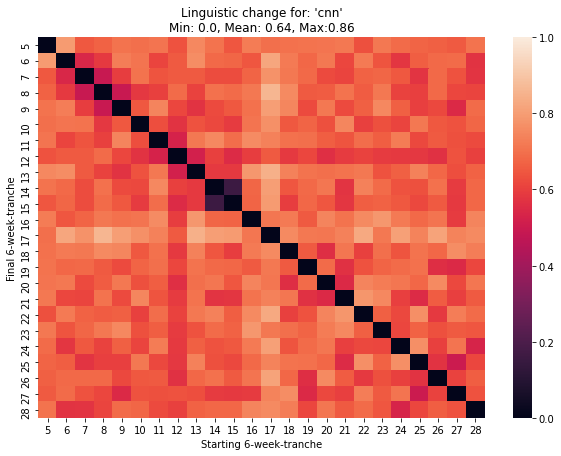
\includegraphics[width=0.32\linewidth]{figures/div_graphs/news-cnn.png} }} ~
    \subfloat[`fox']{{ 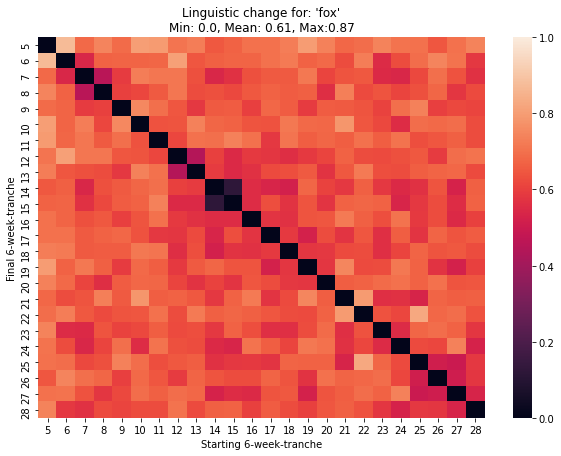
\includegraphics[width=0.32\linewidth]{figures/div_graphs/news-fox.png} }}~ 
    \subfloat[`breitbart']{{ 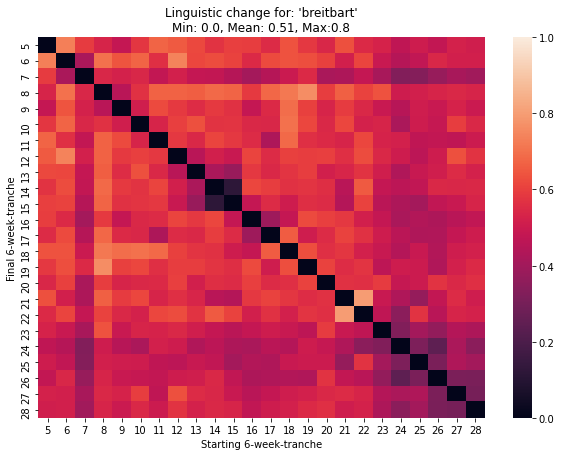
\includegraphics[width=0.32\linewidth]{figures/div_graphs/news-breitbart.png} }}
    
    \caption{Relative Divergence of names of prominent news outlets using aligned word embeddings.}%

    \label{fig:div_news}%

\end{figure}

A salient highlight of President Trump's term has been his frequent attacks on news media outlets, charging them as the 'enemy of the people', of having a vendetta against him, going so far as to institute a list of 'Fake News' award winners. This messaging has had significant success within his base, furthering a partisan re-framing of institutions and working to de-legitimize them. The multiple and varying references to \texttt{cnn} -- albeit in different contexts, since they report on a multitude of issues -- seem like a strong indicator of their centrality to the conversations in the subreddit. The spike in divergence values in period 17 refer to the incident where President Trump re-tweeted a video of attacking CNN.  

On the other hand, President Trump has also expertly tapped into the right-wing media ecosystem to amplify his message. He has made several announced appearances on talk shows hosted by Fox News to chime in on policy. Steve Bannon, chief editor of Breitbart News, was a key figure in the election campaign and was appointed Chief Strategist after the election win, at par with the Chief of Staff \citep{noauthor_donald_2016}. Breitbart has also been a cornerstone of the alt-right, with its nativist and highly partisan coverage crafted for online amplification, replete with fake news and conspiracy theories. For two important news outlets occupying a similar ideological space, their impressions in the subreddit vary drastically. 

% Divergence of Milo vs Hannity
\begin{figure}[h!]%

    \centering

    \subfloat[`hannity' (Sean Hannity)]{{ 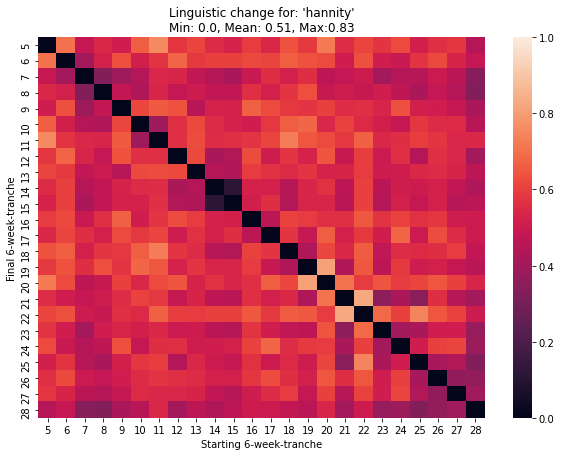
\includegraphics[width=0.32\linewidth]{figures/div_graphs/news-hannity.png} }} ~
    \subfloat[`milo' (Milo Yiannopoulos)]{{ 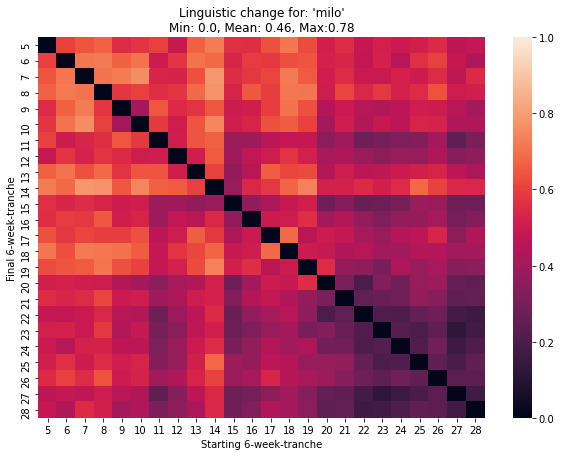
\includegraphics[width=0.32\linewidth]{figures/div_graphs/news-milo.png} }} 
    
    \caption{Relative Divergence of prominent media figures on the right using aligned word embeddings.}%

    \label{fig:div_milo}%

\end{figure}
%--------------------------------------------------------%

\texttt{fox}'s relative divergence map varies in a form similar to that of \texttt{cnn}, while \texttt{breitbart} is likely used in fewer contexts. For the latter, we notice a high change in context at period 22, followed by a period of lower divergence, indicating a stabilization and narrowing of context. The relative fortunes of Fox and Breitbart indicate a shift in attention of the subreddit's sources, with Fox taking on a markedly different role from the first month of the presidency. This shift away from Breitbart is captured well in the subreddit's references to \texttt{milo}, i.e. Milo Yiannopoulos, alt-right provocateur and former editor of Breitbart News. Yiannopoulos's decline as the darling of the alt-right -- following his remarks on pedophilia and child sexual abuse -- tracks with the muted attention of Breitbart in the subreddit, an indicator of weakening influence. 

%--------------------------------------------------------%



\subsubsection*{Salience of Clinton's e-mails and the Russia Investigation}

In Figure \ref{fig:div_emails}, we notice that the term \texttt{email} first changes significance in period 8 and continues to change until period 11. The context stabilizes in periods 16-18. These changes track closely to those of \texttt{russia}, which is to be expected, given Russia's role in the controversy. The timing of these changes coincide with the investigations into Russian interference in the 2016 US elections. These terms both have a high maximum value of divergence, indicating the possibly polysemous nature in which they're being used. The more muted nature of \texttt{hack} is a stronger indicator of the e-mail controversy, owing to its usage in association with the John Podesta email hack. Compared to the use of \texttt{leak} which could refer to other administrative leaks with varying contexts in the Trump government, it has much greater variation in usage. 

Figure \ref{fig:div_scandals} shows us how the context around the impeachment investigations have changed over time. We notice a spike in divergence in period 11 for \texttt{impeach}, right after the election, indicating how this was a hot-button issue immediately. Additionally, we notice a rise in divergence in period 13 for \texttt{hoax}, pointing to President Trump's claims calling Russian interference in the elections a hoax \citep{noauthor_trump_2019}. We see a higher and more disperse spread of divergence for \texttt{hunt}, beginning in period 17, when President Trump claimed that the Democrats were engaged in a 'witch hunt' \citep{noauthor_donald_nodate}. 

% Divergence of scandals
\begin{figure}[h!]%

    \centering

    \subfloat[`impeach' (Impeachment)]{{ 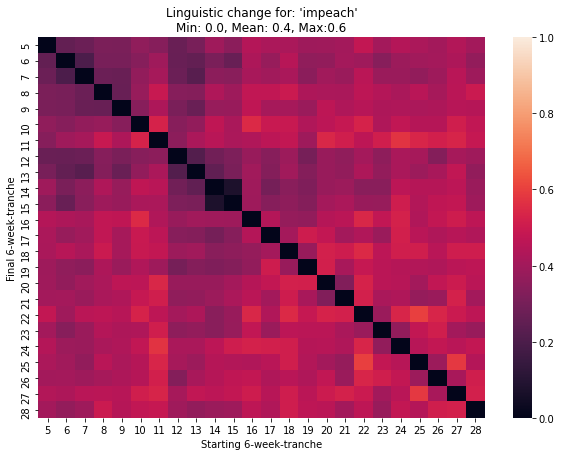
\includegraphics[width=0.28\linewidth]{figures/div_graphs/scandals-impeach.png} }} ~
    \subfloat[`hoax' (Russia hoax)]{{ 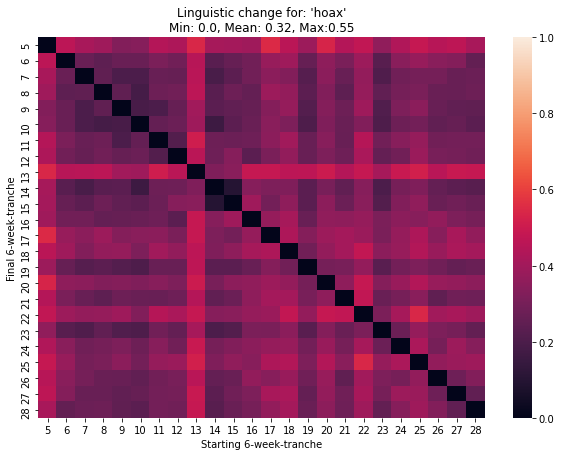
\includegraphics[width=0.28\linewidth]{figures/div_graphs/scandals-hoax.png} }} ~
    \subfloat[`hunt' (`Witch Hunt')]{{ 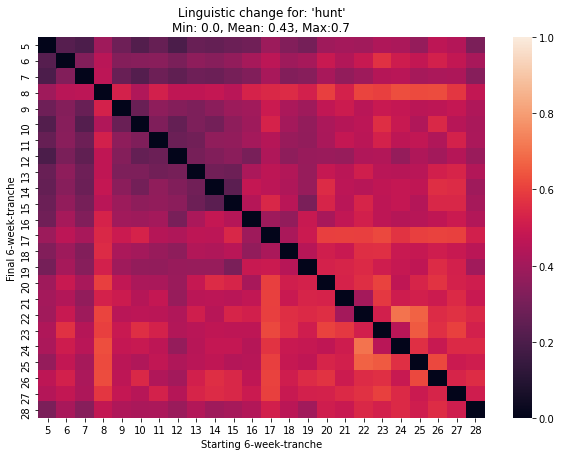
\includegraphics[width=0.28\linewidth]{figures/div_graphs/scandals-hunt.png} }}
    
    \caption{Relative Divergence of words related to Trump's scandals using aligned word embeddings.}%

    \label{fig:div_scandals}%

\end{figure}

% Divergence of e-mails
\begin{figure}[t]%

    \centering

    \subfloat[`email']{{ 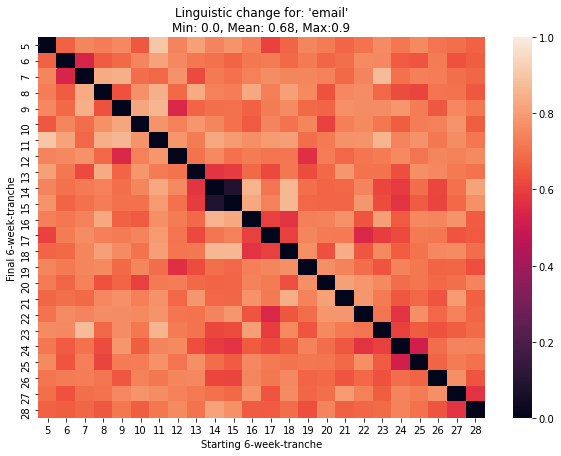
\includegraphics[width=0.28\linewidth]{figures/div_graphs/emails-email.png} }} ~
    \subfloat[`russia']{{ 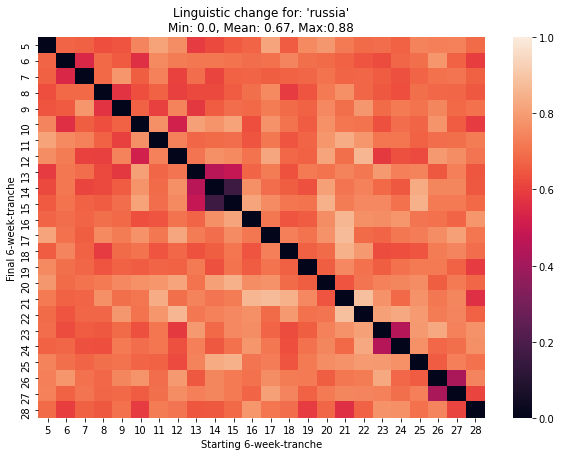
\includegraphics[width=0.28\linewidth]{figures/div_graphs/emails-russia.png} }}
    
    \subfloat[`hack']{{ 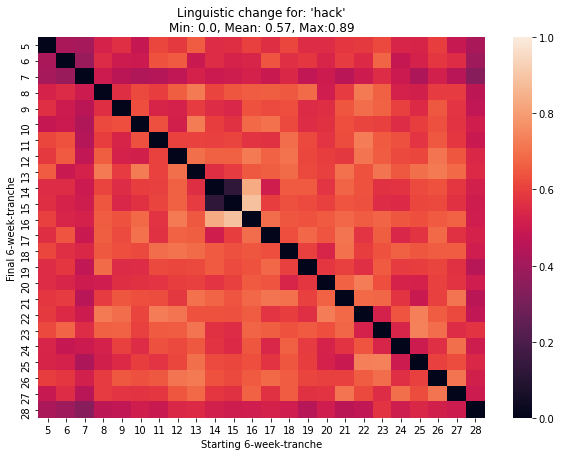
\includegraphics[width=0.28\linewidth]{figures/div_graphs/emails-hack.png} }} ~
    \subfloat[`leak']{{ 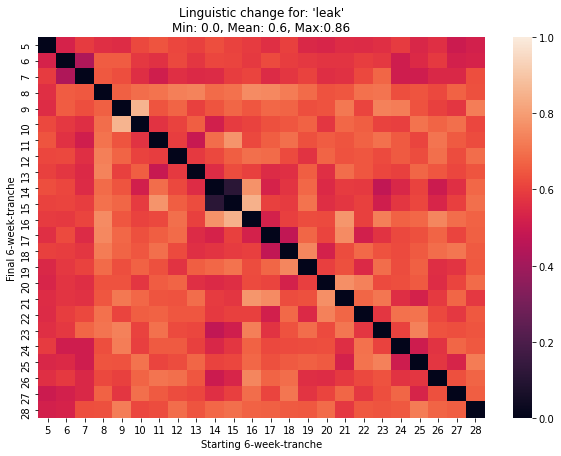
\includegraphics[width=0.28\linewidth]{figures/div_graphs/emails-leak.png} }}
    
    \caption{Relative Divergence of words related to Clinton's e-mail controversy using aligned word embeddings.}%

    \label{fig:div_emails}%

\end{figure}
%---------------------------------------------------------%

\subsubsection*{Tracking tariffs and the trade war}

President Trump's focus on 'Make America Great Again' has also translated into renewed attention on American manufacturing, and the the effect of free-trade agreements on jobs in America. As he tried to publicly push companies to move jobs back to the US, he also criticized past administrations for crafting unfavourable trade deals with China. This soon morphed into a trade war with China, with escalating tariffs levied by both sides.  We notice the first change in the context surrounding the word \texttt{tariff} in period 13, in the first quarter of the presidency, followed by no change for an extended period. This is indicative of a significant change in rhetoric in period 13, until period 23. The change in period 23 is matched by those for words \texttt{trade} and \texttt{china}. This period included a serious escalation of the trade war with China. 

% Divergence of trade
\begin{figure}[b]%

    \centering

    \subfloat[`China']{{ 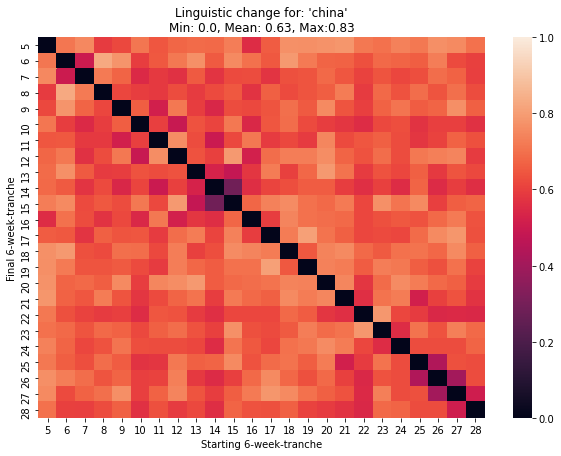
\includegraphics[width=0.265\linewidth]{figures/div_graphs/trade-china.png} }} ~
    \subfloat[`tariff']{{ 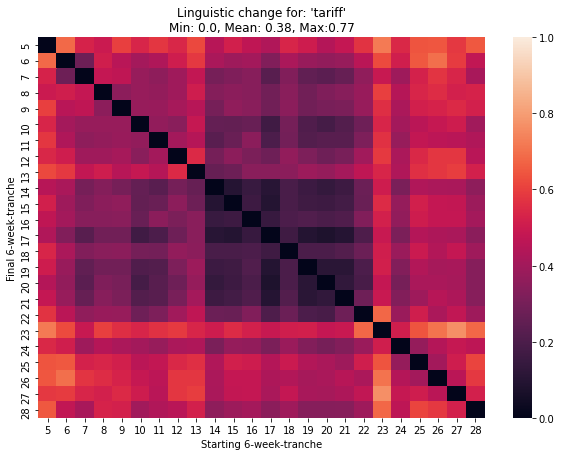
\includegraphics[width=0.265\linewidth]{figures/div_graphs/trade-tariff.png} }} ~
    \subfloat[`trade']{{ 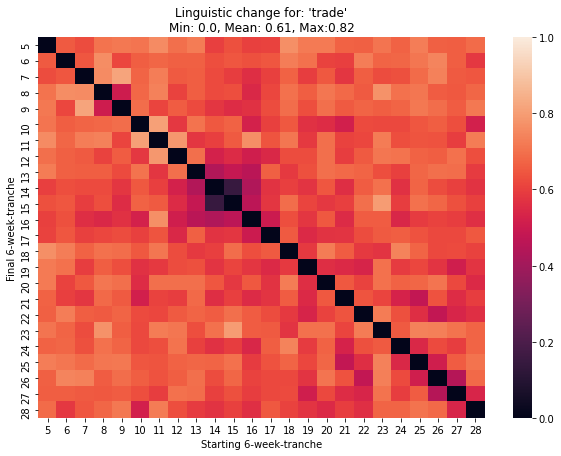
\includegraphics[width=0.265\linewidth]{figures/div_graphs/trade-trade.png} }} 
    
    \caption{Relative Divergence of words related to Trump's trade war with China using aligned word embeddings.}%

    \label{fig:div_trade}%

\end{figure}

%--------------------------------------------------------%


\subsection*{Using Projections of Word Embeddings to understand relative positions}

\subsubsection*{Changing associations of political figures}

Figure \ref{fig:proj_parties} provides a projection of political names and entities onto dimensions of security, trade, ideology, region, economy, and race. I select the names of the candidates in the 2016 US elections and the names of the political parties, to understand how their relative positions on these political dimensions change over time in the subreddit. This helps us understand how the community's language and context around these figures, and by extension their perception of these entities, has shifted over time. 

On the `Security' dimension in figure \ref{fig:proj_parties}, we notice how \texttt{trump} ranks consistently high relative to all other entities. \texttt{clinton} moves towards the lower end of the dimension in the month of the election, indicating how the subreddit viewed her as being weak on Security issues. \texttt{democrat} is consistently on the lower dimension (weak security) in all but one window, that of the election. I interpret this as Clinton's fall from relevance as the opposition to President Trump after his election. 

On questions of Ideology, we notice \texttt{trump} and even \texttt{democrat} not being fixed on the dimension, with only \texttt{republican} being static. We also notice how \texttt{bernie} and \texttt{stein} consistently represent the opposite of the Republican ideology. This latter observation should not be surprising -- Bernie Sanders and Jill Stein have been purists for the duration of their political careers, and stand in stark opposition to the Republicans. Interestingly, in the  period of the election, \texttt{stein} moves to the center while \texttt{clinton} moves to the extreme -- a strong indicator of how perceptions in the lead-up to the elections were vastly different from other periods.

On questions of the Economy, \texttt{trump} loads heavily on the poor or non-elite end of the dimension, affirming the perception of his anti-establishment credentials.  \texttt{bernie} occupies a similar position. \texttt{clinton} is positioned on the `rich' end of the dimension in the month of the election, showcasing how her established pedigree came to the fore in that period. On the dimension of Race, \texttt{trump} shows up close to the extreme in two windows: Super Tuesday 2016, and August 2017 during the Charlottesville attack. Both these periods were dominated by strong racial and ethno-nationalist messaging by Trump and his staff.  

% Projection of candidate names 
\begin{figure}[h]%
    \centering

    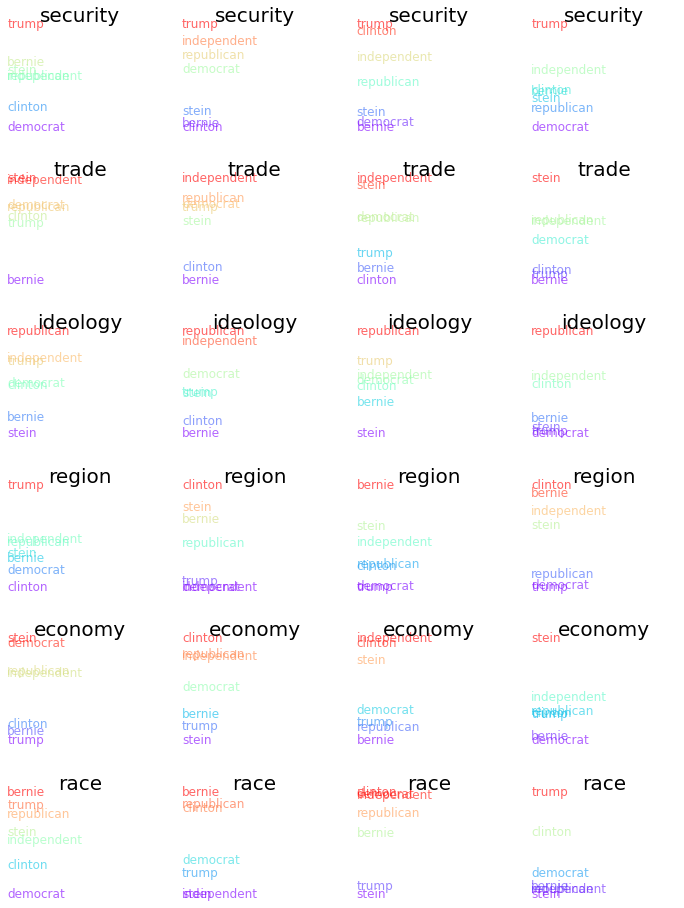
\includegraphics[width=0.95\textwidth]{figures/proj-candi.png}

    \caption{Projection of Candidate and Party names on dimensions of Security (strong-weak), Trade (local-global), Ideology (right-left), Region (urban-rural), Economy (rich-poor), and Race (american-immigrant). \\ From left to right, each projection refers to the time-window including (1) Super Tuesday in March 2016, (2) Elections in November 2016, (3) the first quarter of the presidency in Feb-Mar 2017, and (4) the `Unite the Right' rally in Charlottesville, August 2017}%

    \label{fig:proj_parties}%

\end{figure}
%--------------------------------------------------------%

\subsubsection*{Consistent perceptions of news outlets}

Figure \ref{fig:proj_media} provides a projection of news outlets -- print and Television -- on the aforementioned dimensions. I split them into these categories to disambiguate the different positions they take, and to examine equivalent pairs, like CNN-Fox, and NYT-Breitbart.

On the `Security' dimension in figure \ref{fig:proj_media}a, Fox News consistently ranks high relative, with MSNBC and CNN occupying the `weak' end of the dimension. The distance between Fox an the rest of the outlets from the second window onwards is indicative of the extreme posturing characteristic of their content. Fox also projects heavily on the `conservative' end of the ideology dimension, but it's surprising to see CNN show up there in the third window (first quarter of the Presidency).  

On matters of `Trade', MSNBC and CNN load heavily on the `global' end of the dimension. Other outlets like CBS and ABC promptly occupy the center on this dimension too. MSNBC and CNN occupy similar positions again on the `Economy' dimension, with the community perceiving them to be more closely associated with the `poor' end of the dimension. On questions of `Race' again, CNN stays reliably to the `immigrant' end of the dimension.

The consistency of the results persist with print news outlets too. National Review stakes its position as a conservative hawk on the Security dimension, its relative position far away from the other print outlets. The New York Times, Washington Post, and Wall Street Journal regularly load heavier on the `weak' end of this dimension, with Breitbart closer to the Review. The conservative nature of the Review persists on the Trade dimension, along with more globalist positions taken by the Times, Post and Journal.


% Projection of News outlets
\begin{figure}[t]%

    \centering

    \subfloat[Television News Media. Includes `MSNBC', `CNN', `ABC News', `CBS News', and `Fox News'.]{{ 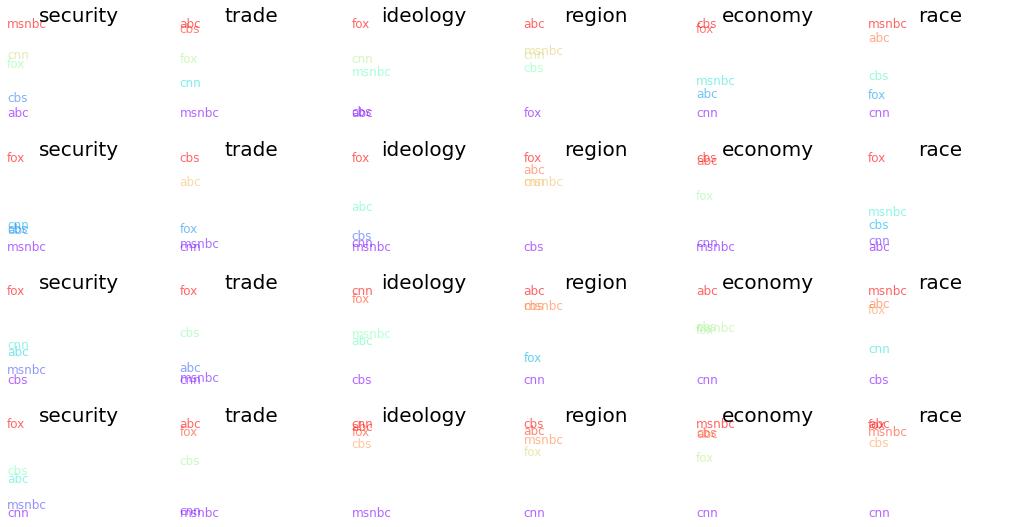
\includegraphics[height=0.38\textheight]{figures/proj-tv_news.png} }}
    
    \subfloat[Print News Media. Includes `New York Times', `Washington Post', `Wall Street Journal', `National Review', and `Breitbart'.]{{ 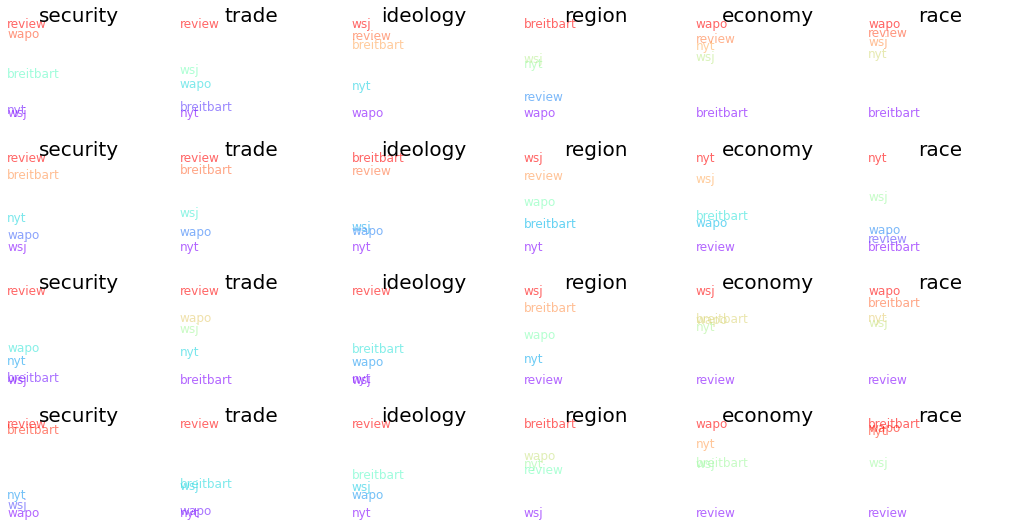
\includegraphics[height=0.38\textheight]{figures/proj-news.png} }}%

    \caption{Projection of Television and Print media outlets on dimensions of Security (strong-weak), Trade (local-global), Ideology (right-left), Region (urban-rural), Economy (rich-poor), and Race (american-immigrant). \\ From top to bottom, each projection refers to the time-window including (1) Super Tuesday in March 2016, (2) Elections in November 2016, (3) the first quarter of the presidency in Feb-Mar 2017, and (4) the `Unite the Right' rally in Charlottesville, August 2017}%

    \label{fig:proj_media}%

\end{figure}
%--------------------------------------------------------%









% \begin{equation}
% \label{eq:emc}
% e = mc^2
% \end{equation}

